	\documentclass[10pt,oneside]{CBFT_book}
	% Algunos paquetes
	\usepackage{amssymb}
	\usepackage{amsmath}
	\usepackage{graphicx}
	\usepackage{libertine}
	\usepackage[bold-style=TeX]{unicode-math}
	\usepackage{lipsum}

	\usepackage{natbib}
	\setcitestyle{square}

	\usepackage{polyglossia}
	\setdefaultlanguage{spanish}


	\usepackage{CBFT.estilo} % Cargo la hoja de estilo

	% Tipografías
	% \setromanfont[Mapping=tex-text]{Linux Libertine O}
	% \setsansfont[Mapping=tex-text]{DejaVu Sans}
	% \setmonofont[Mapping=tex-text]{DejaVu Sans Mono}

	%===================================================================
	%	DOCUMENTO PROPIAMENTE DICHO
	%===================================================================

\begin{document}

% =================================================================================================
\chapter{Ondas planas}
% =================================================================================================

Lejos de las fuentes de campo las ecuaciones de Maxwell son
\begin{align*}
	\divem{E} = 0 \qquad \qquad &\rotorm{E} = -\frac{1}{c}\dpar{\vb{B}}{t} \\
	\divem{B} = 0 \qquad \qquad &\rotorm{B} = \frac{1}{c}\dpar{\vb{E}}{t}
\end{align*}

Podemos derivar con respecto al tiempo en cada ecuación de rotor y reemplazar con la otra
de manera que
\[
	\rotorm{(\rotorm{B})} = \frac{1}{c}\dpar{}{t}\left(-\frac{1}{c}\dpar{\vb{B}}{t} \right)
	= \Nabla(\divem{B}) - \nabla^2 \vb{B}
\]
\[
	\rotorm{(\rotorm{E})} = -\frac{1}{c}\dpar{}{t}\left(\frac{1}{c}\dpar{\vb{E}}{t} \right)
	= \Nabla(\divem{E}) - \nabla^2 \vb{E}
\]
y esto nos lleva a 
\[
	\nabla^2 \vb{B} - \frac{1}{c^2}\dpar[2]{\vb{B}}{t} = 0 \qquad 
	\nabla^2 \vb{E} - \frac{1}{c^2}\dpar[2]{\vb{E}}{t} = 0
\]
dos sendas ecuaciones de onda para \vb{E} y \vb{B}. Pero es sabido que la solución de
\[
	\nabla^2 \psi - \frac{1}{c^2} \dpar[2]{\psi}{t} = 0
\]
es
\[
	\psi = A\euler^{i(\pe{k}{x}-\omega t)} + B\euler^{i(\pe{k}{x}-\omega t)}
\]
de modo que podemos postular como soluciones para nuestras ecuaciones de onda a
\[
	\vb{E} = \vec{\mathbb{E}}_0 \euler^{i(\pe{k}{x}-\omega t)} \qquad 
	\vb{B} = \vec{\mathbb{B}}_0 \euler^{i(\pe{k}{x}-\omega t)}
\]

Se tiene además que $\vb{k} = k \hat{n}$ da a través de $\hat{n}$ la dirección de
propagación de la onda. El número de onda $k$ podrá ser complejo lo cual refleja
atenuación. Las características del medio entran a través de
\[
	k = \sqrt{\mu\epsilon} \frac{\omega}{c}
\]
\notamargen{Acá hay que hacer las cuentas para demostrar todo esto que acá se
dice sin más.}
Por su parte $\vec{\mathbb{E}}_0$ y $\vec{\mathbb{B}}_0$ son complejos uniformes y
podrán dar desfasajes.

Al utilizar las ecuaciones de divergencia sobre las soluciones se obtiene que 
\[
	\hat{n}\cdot \vec{\mathbb{E}}_0 = 0 \qquad \hat{n}\cdot \vec{\mathbb{B}}_0 = 0
\]
de manera que las ondas se propagan perpendicularmente a los campos, por ello las
ondas electromagnéticas son transversales.

Utilizando las ecuaciones de rotor se llega a la importante relación 
\[
	\vec{\mathbb{B}}_0 = \sqrt{\mu\epsilon} \hat{n} \times \vec{\mathbb{E}}_0
\]
de modo que los vectores $\vec{\mathbb{E}}_0$ y $\vec{\mathbb{B}}_0$ también son perpendiculares.
Si el vector $\vb{k} \in \mathbb{R}$ entonces $\vec{\mathbb{E}}_0$ y $\vec{\mathbb{B}}_0$
tienen la misma fase.

En el vacío o en un medio LIH los campos \vb{E} y \vb{B} estarán en fase.
Asimismo
\[
	\vb{S} \parallel \hat{n}
\]
pues $\vb{S} \propto \pv{E}{H} $.

En un medio anisótropo $\divem{D}=\divem{}(\epsilon \vb{E}) = 0$ siendo $\epsilon$ un tensor.
Allí $\vec{\mathbb{E}}_0 \cdot \hat{n} \neq 0$ salvo que $\epsilon$ estee diagonalizado y
$\vb{E} \parallel$ al eje principal.

Notemos que $\vb{E},\vb{B}$ y $\hat{n}$ forman una terna derecha.

\subsection{Sobre complejos}
\[
	\mathcal{R}(A) = \frac{1}{2}( A + A^* )	\qquad \text{con} \; A \in \mathbb{C}
\]
Sean 
\[
	\vb{A}(\vb{x},t) = \vb{A}(\vb{x})\euler^{-i\omega t} \qquad \qquad 
			\vb{B}(\vb{x},t) = \vb{B}(\vb{x})\euler^{-i\omega t}
\]
siempre trabajaremos en general con dependencias temporales armónicas y metemos $\euler^{i\pe{k}{x}}$ en el 
módulo $vb{A}_0$ que pasa a depender de $\vb{x}$.

Los campos físicos son siempre la parte real de las expresiones complejas.
\[
	\mathcal{R}(\vb{A} + \vb{B}) = \mathcal{R}( \vb{A} ) + \mathcal{R}( \vb{B} )
\]
con operaciones lineales es lo mismo tomar parte real antes o después.
\[
	\mathcal{R}(\vb{A}.\vb{B}) \neq  \mathfrak{R}( \vb{A} ) + \mathcal{R}( \vb{B} )
\]
con operaciones no lineales no es lo mismo.
Para hacer producto necesito tomar la parte real de cada factor y entonces
\[
	\mathfrak{R}( \vb{A} ).\mathfrak{R}( \vb{B} ) = \frac{1}{2}\mathfrak{R}( \vb{A}.\vb{B}^* + 
			\vb{A}.\vb{B} \euler^{ -i 2 \omega t })
\]

Pero como en las aplicaciones estaré interesado en el promedio sobre un número entero de períodos,
\[
	\langle \vb{A} \vb{B} \rangle = \langle \mathfrak{R}( \vb{A} ). \mathfrak{R}( \vb{B} ) \rangle =
			\frac{1}{2} \mathfrak{R} ( \vb{A}.\vb{B}^* )
\]

\subsection{Poynting promedio y energías promedio}

Los campos \vb{E} y \vb{H} en ondas electromagnéticas toman la forma 
\[
	\vb{E} = \vec{\mathbb{E}}(\vb{x})\euler^{-i\omega t} \qquad 
	\vb{H} = \vec{\mathbb{H}}(\vb{x})\euler^{-i\omega t}
\]
de manera que 
\[
	\vb{S}( \vb{x},t ) = \frac{c}{4\pi} \frac{1}{2} \re( \vec{\mathbb{E}} \times \vec{\mathbb{H}}^* + 
		\vec{\mathbb{E}} \times \vec{\mathbb{H}} \euler^{-i2\omega t})
\]
\[
	\langle \vb{S}( \vb{x},t ) \rangle = \frac{c}{8\pi} \re( \vec{\mathbb{E}} \times \vec{\mathbb{H}}^* ) 
\]

En un MLIH es 
\[
	\vec{\mathbb{B}} = \sqrt{ \mu \epsilon } \hat{n} \times \vec{\mathbb{E}} \qquad\qquad 
	\vec{\mathbb{H}} = \sqrt{ \frac{\epsilon}{\mu } } \hat{n} \times \vec{\mathbb{E}}
\]
donde usamos que $\vb{H} = \vb{B}/\mu$
\[
	\langle \vb{S}( \vb{x},t ) \rangle = \frac{c}{8\pi} \re( \vec{\mathbb{E}} \times 
		\sqrt{\frac{\epsilon}{\mu}}(\hat{n} \times \vec{\mathbb{E}})^* )
\]
\[
	\langle \vb{S}( \vb{x},t ) \rangle = \frac{c}{8\pi} \sqrt{\frac{\epsilon}{\mu}} 
		( \hat{n} (\vec{\mathbb{E}}\cdot\vec{\mathbb{E}}^*) - 
		\vec{\mathbb{E}}^*(\vec{\mathbb{E}}\cdot\hat{n}) )
\]
y finalmente
\[
	\langle \vb{S}( \vb{x},t ) \rangle = \frac{c}{8\pi} 
		\sqrt{\frac{\epsilon}{\mu}}|\vec{\mathbb{E}}|^2 \hat{n}
\]
que es el vector de Poynting para ondas en MLIH.
\[
	U(\vb{x},t) = \frac{1}{8\pi}( \pe{H}{B} + \pe{E}{D} )
\]
\[
	\langle U(\vb{x},t) \rangle = \frac{1}{8\pi} \frac{1}{2} \re ( 
	\vec{\mathbb{H}}\cdot\vec{\mathbb{B}}^* + \vec{\mathbb{E}}\cdot\vec{\mathbb{D}}^* )
\]
\[
	\langle U(\vb{x},t) \rangle = \frac{1}{16\pi}
		\re ( \frac{1}{\mu} |\vec{\mathbb{B}}|^2 + \epsilon |\vec{\mathbb{E}}|^2 ) =
		\frac{1}{8\pi} |\vec{\mathbb{E}}|^2
\]
puesto que 
\[
	|\vec{\mathbb{B}}|^2 = \mu\epsilon |\vec{\mathbb{E}}|^2,	
\]
y entonces la densidad de energía promedio es
\[
		\langle U(\vb{x},t) \rangle = \frac{1}{8\pi} |\vec{\mathbb{E}}|^2.
\]

% =================================================================================================
\section{Polarización de ondas}
% =================================================================================================

Una onda plana bien general en $\hat{n}$ es 
\[
	\vb{E}( \vb{x},t )=(\hat{\epsilon}_1 \vec{\mathbb{E}}_1 + 
			\hat{\epsilon}_2\vec{\mathbb{E}}_2) \euler^{i( \pe{k}{x} -\omega t)}
\]

\begin{figure}[htb]
	\begin{center}
	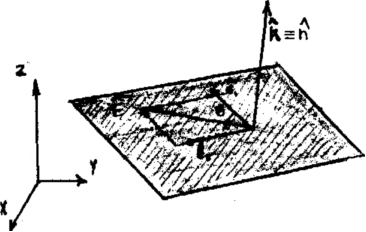
\includegraphics[width=0.4\textwidth]{images/fig_ft1_polariz.pdf}	 
	\end{center}
	\caption{}
\end{figure} 

Si $\vec{\mathbb{E}}_1,\vec{\mathbb{E}}_2$ están en fase entonces $\vb{E}( \vb{x},t )$ está linealmente
polaridaza con $\theta$ fijo.
Es como que \vb{E} viaja siempre por el mismo andarivel, oscilando. Las amplitudes 
$\vec{\mathbb{E}}_1,\vec{\mathbb{E}}_2$ son complejos para permitir la diferencia de fase entre componentes.

Si $\vec{\mathbb{E}}_1,\vec{\mathbb{E}}_2$ tienen fase arbitraria entonces $\vb{E}( \vb{x},t )$ está elípticamente 
polarizada.

Si $|\vec{\mathbb{E}}_1|=|\vec{\mathbb{E}}_2|$ y la fase es $\pi/2$ entonces $\vb{E}( \vb{x},t )$ está circularmente 
polarizada.

\[
	\vec{\mathbb{E}}_2 = \vec{\mathbb{E}}_1 \euler^{i \pi/2} =\vec{\mathbb{E}}_1 i
\]
entonces
\[
	\vb{E}( \vb{x},t )= \vec{\mathbb{E}}_1 (\hat{\epsilon}_1  \pm \hat{\epsilon}_2 )
				\euler^{i( \pe{k}{x} -\omega t)}	
\]
donde el $+$ corresponde a $\mathcal{C}^+$ antihoraria y el $-$ a horaria. Nos definimos por comodidad,
\[
	\hat{\epsilon}_+ \equiv \frac{\hat{\epsilon}_1 + i \hat{\epsilon}_2 }{\sqrt{2}} \qquad\qquad 
	\hat{\epsilon}_- = \frac{\hat{\epsilon}_1 - i \hat{\epsilon}_2 }{\sqrt{2}}
\]
una base de polarizaciones. Se cumplen
\[
	\hat{\epsilon}_\pm \cdot \hat{\epsilon}_\mp^* = 0 \qquad \qquad 
	\hat{\epsilon}_\pm \cdot \hat{\epsilon}_\pm^* = 1
\]
\[
	\hat{\epsilon}_1 = \sqrt{2}( \hat{\epsilon}_+ + i \hat{\epsilon}_- ) \qquad \qquad 
	\hat{\epsilon}_2 = \sqrt{2}( \hat{\epsilon}_+ - i \hat{\epsilon}_- )
\]
luego cualquier polarización se puede escribir como combinación lineal de $\mathcal{C}^+$ y $\mathcal{C}^-$.
Entonces una onda plana general es
\[
	\vb{E}( \vb{x},t )=(\hat{\epsilon}_+ \vec{\mathbb{E}}_+ + 
			\hat{\epsilon}_-\vec{\mathbb{E}}_-) \euler^{i( \pe{k}{x} -\omega t)}
\]

Una onda que rebota en un espejo transfiere impulso lineal. Una onda $\mathcal{C}$ lleva \vb{L} pero no lo transfiere 
en un rebote perfecto. Por ser \vb{L} un vectorial axial (pseudovector) el reflejo es equivalente a una simetría del 
sistema.

Tenemos dos base entonces $\{ \hat{\epsilon}_1 ,\hat{\epsilon}_2 \}$ y $\{ \hat{\epsilon}_+ ,\hat{\epsilon}_- \}$.
Además,
\[
	\frac{\vec{\mathbb{E}}_-}{\vec{\mathbb{E}}_+} = r\euler^{i\alpha} 
\]
si $r = \pm 1, \alpha=0 $ entonces estamos frente a linealmente polarizada.

% =================================================================================================
\section{Reflexión y refracción de ondas en medios}
% =================================================================================================

Partimos de una onda
\[
	\vb{E}( \vb{x},t )= \vec{\mathbb{E}}_0 \euler^{i( \pe{k}{x} -\omega t)}
\]
donde 
\[
	k = \sqrt{\mu\epsilon} \frac{\omega}{c} = \frac{\omega}{v}
\]
siendo $v$ la velocidad en el medio. Los índices de refracción serán 
\[
	n = \sqrt{\mu \epsilon} \qquad  n' = \sqrt{\mu' \epsilon'}
\]
de tal suerte que los campos son 
\[
	\vb{B} = \frac{\sqrt{\mu\epsilon}}{k} \; \pv{k}{E} \qquad \quad 
		\vb{H} = \sqrt{\frac{\epsilon}{\mu}} \frac{1}{k} \; \pv{k}{E}
\]
\begin{figure}[htb]
	\begin{center}
	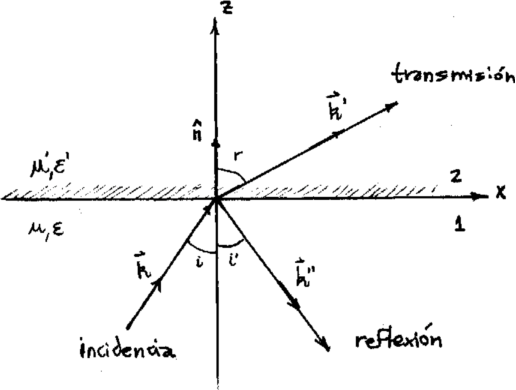
\includegraphics[width=0.7\textwidth]{images/fig_ft1_reflex1.pdf}	 
	\end{center}
	\caption{}
\end{figure} 

y tenemos 

\[
	|\vb{k}| = |\vb{k}''| \qquad \text{pues} \quad \mu''= \mu,\; \epsilon''=\epsilon
\]

Utilizando las condiciones de contorno llegamos a
\[
	\omega t = \omega' t = \omega'' t
\]
\[
	\pe{k}{x}\:|_{z=0} = \pe{k'}{x}\:|_{z=0}  = \pe{k''}{x}\:|_{z=0} 
\]
La existencia de condiciones de contorno en $z=0$ que deben ser satisfechas en todo $t$ en todo punto $(x,y)$ lleva a 
todos los factores de fase iguales en $z=0$. Se debe tener \vb{B} normal continuo y \vb{D} normal continuo también, lo 
cual viene de $\divem{B}=0$ y $\divem{D}=0$.

La frecuencia $\omega$ es la misma para el medio 1 y el medio 2 pues $\lambda_1 \neq \lambda_2$.

Los tres vectores $\vb{k}, \vb{k}', \vb{k}''$ están en un mismo plano, entonces 
\[
	k \sin(i) = k' \sin(r) = k'' \sin(i'),
\]
y se deducen las consecuencias
\[
	n \sin (i) = n' \sin(i') \qquad \text{Ley de Snell},
\]
\[
	i = i' \qquad \text{Ley de reflexión}
\]
Luego se plantean los contornos 
\[
	D_{\hat{n}} : \qquad [ \vb{D}_2 - \vb{D}_1 ]\cdot\hat{n} = 0 \qquad \rightarrow  \qquad 
		[ \epsilon'\vb{E}_0^{'} - \epsilon (\vb{E}_0 + \vb{E}_0^{''} )  ]\cdot\hat{n} = 0
\]
\[
	E_{\hat{t}} : \qquad \hat{n} \times [ \vb{E}_2 - \vb{E}_1 ] = 0 \qquad \rightarrow \qquad 
		\hat{n} \times [ \vb{E}_0^{'} - (\vb{E}_0 + \vb{E}_0^{''} )  ]  = 0
\]
\[
	B_{\hat{n}} : \qquad  [ \vb{k}' \times \vb{E}_0^{'} - ( \vb{k} \times \vb{E}_0 + 
			\vb{k}'' \times \vb{E}_0^{''} )  ]\cdot\hat{n} 
\]
\notamargen{Igual a cero esto?}
\[
	H_{\hat{t}} : \qquad  \hat{n} \times \left[ \frac{1}{\mu'}\vb{k}' \times \vb{E}_0^{'} - 
			\frac{1}{\mu}( \vb{k} \times \vb{E}_0 + \vb{k}'' \times \vb{E}_0^{''} ) \right]  = 0
\]
de manera que 
\[
	\vb{B} = \frac{\sqrt{\mu\epsilon}}{k} \pv{k}{E} = \frac{c}{\omega} \pv{k}{E} \qquad \qquad 
	\vb{H} = \frac{c}{\mu \omega } \pv{k}{E}
\]

donde $c/\omega$ es el mismo para ambos medios.

Aplicando diligentemente los contornos se llega a las {\it relaciones de Fresnel} que son los cocientes de las 
amplitudes relativas.

Usando $\mu \sim 1$ (válido para medios transparentes) tenemos

\[
	TE \qquad \qquad TM
\]
\[
	\frac{E_0^{''}}{E_0} = -\frac{\sin(i-r)}{\sin(i+r)} \qquad \qquad 
	\frac{E_0^{''}}{E_0} = \frac{\tan(i-r)}{\tan(i+r)} 
\]
\[
	\frac{E_0^{''}}{E_0} = 1 + \frac{\sin(r-i)}{\sin(i+r)} \qquad \qquad 
	\frac{E_0^{''}}{E_0} = \frac{2 \sin(r)\cos(i)}{\sin(i+r)\cos(i-r)} 
\]
\begin{figure}[htb]
	\begin{center}
	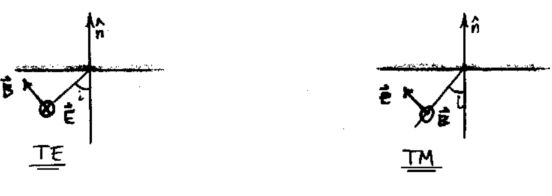
\includegraphics[width=0.7\textwidth]{images/fig_ft1_reflex2.pdf}	 
	\end{center}
	\caption{}
\end{figure} 

\notamargen{frecuencias ópticas $\mu'/\mu = 1$}.

Si $i \sim 0$ entonces TE y TM son similares a menos de un signo.

\subsubsection{Polarization (Brewster angle)}

Es un $i_B$ tal que no hay onda \vb{E} reflejada (en TM),
\[
	E_0^{''} = 0,
\]
puest $\tan( i + r) \to \infty$
\[
	i_b = atan \left( \frac{n'}{n}\right) ,
\]
pues $ i_B + r = \pi/2$ entonces 
\[
	\frac{n}{n'}\sin(i_B) = cos(i_B) \rightarrow i_b = atan \left( \frac{n'}{n}\right),
\]
Sirve para producir luz polarizada linealmente.

\begin{figure}[htb]
	\begin{center}
	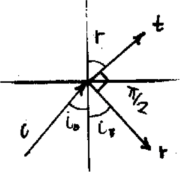
\includegraphics[width=0.4\textwidth]{images/fig_ft1_reflex3.pdf}	 
	\end{center}
	\caption{}
\end{figure} 

Atención, pero 
\[
	\vb{S}_i \neq \vb{S}_r + \vb{S}_t ,
\]
pues \vb{S} no está relacionado linealmente con \vb{E}, \vb{B}, y lo que sí vale es
\[
	\vb{S}_i \cdot \hat{n} = \vb{S}_r \cdot \hat{n} + \vb{S}_t \cdot \hat{n} 
\]


\subsubsection{Reflexión interna total}

Sea $ n_{inc} > n_{trans} $. Entonces se da que
\[
	n \sin(i) = n'\sin(r),
\]
\[
	\frac{n}{n'} \sin(i) = \sin(r),
\]
y el LHS es mayor igual a 1 para algunos $i$. Existe un ángulo límite 
\[
	\sin(r) = 1 = \frac{n}{n'} \sin(i) 
\]
\[
	i_0 = asin\left( \frac{n'}{n} \right)
\]
de manera que si $i \geq i_0$ entonces $\sin(r) > 1$ y se debe tener un $r\in \mathbb{C}$.

\begin{figure}[htb]
	\begin{center}
	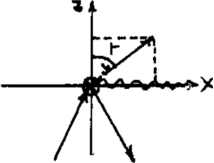
\includegraphics[width=0.4\textwidth]{images/fig_ft1_reflex4.pdf}	 
	\end{center}
	\caption{}
\end{figure} 

Si $\sin(r)>1$ se tiene $\sin(r)^2 > 1$ y como por teorema de Pitágoras es 
\[
	\cos(r)^2 = 1 - \sin(r)^2 \rightarrow \cos(r) = i \sqrt{ \sin(r)^2 - 1 }
\]
donde notemos espcialmente que hemos sacado fuera un $\sqrt{-1} = i$ para que el argumento de la raíz sea positivo en 
este caso especial. Luego 
\[
	\cos(r) = i \sqrt{ \frac{n}{n'}\sin(i)^2 - 1 } = i a 
\]
y si $\sin(r) = 1$ entonces $r = \pi/2$.
Entonces
\[
	\euler^{i(\vb{k}\cdot\vb{x})} = \euler^{i(k \cos(r)z + k \sin(r)x)} =
		\underbrace{\euler^{-kaz}}_{\text{atenuación}} 
		\underbrace{\euler^{ik\sin(r)x}}_{\text{propagación}}
\]


% =================================================================================================
\section{Corrientes en conductores}
% =================================================================================================

La continuidad de la carga y la divergencia de \vb{D},
\[
	\divem{J} + \dpar{\rho}{t} = 0 \qquad \qquad \divem{D} = 4\pi \rho,
\]
nos llevan a
\[
	\divem{J} + \frac{1}{4\pi}\Nabla\cdot \dpar{\vb{D}}{t} = 0
\]
\[
	\Nabla\cdot \left( \vb{J} + \frac{1}{4\pi} \dpar{\vb{D}}{t} \right) = 0
\]
y esto lo puedo pensar como una densidad de corriente estacionaria,
\be
	\divem{J}_e = 0
	\label{diver_jcond}
\ee
siendo $\vb{J}_e$ proveniente de un \vb{E'} tal que $\rotorm{E'} \neq 0$.
\notamargen{Un campo irrotacional no puede mantener una corriente estacionaria, necesito
una FEM para ella. La FEM es una fuente de \vb{E} no conservativo.}

Recordando la ley de Ohm microscópica, $\vb{J} = \sigma \vb{E}$ ,
\[
	\vb{D} = \epsilon \vb{E} = \frac{\epsilon}{\sigma} \vb{J}
\]
y esto nos conduce a una ecuación diferencial para \vb{J},
\[
	\vb{J}_e = \vb{J} + \frac{\epsilon}{4\pi\sigma} \dpar{\vb{J}}{t} =
	\left( 1 + \frac{\epsilon}{4\pi\sigma} \dpar{}{t} \right)
\]
y entonces 
\[
	\vb{J} = \vb{J}_e + \vb{J}_0 \euler^{-4\pi\sigma/\epsilon t }
\]
siendo el segundo término del RHS la parte no estacionaria de la corriente. Evidentemente, si $t \to \infty$ esta 
tiende a cero.

Dado que se verifica \eqref{diver_jcond} se tiene 
\[
	-\dpar{\rho}{t} = \divem{J}_0 \euler^{-4\pi \sigma/\epsilon t}
\]
y definimos un tiempo de relajación
\[
	\tau = \frac{\epsilon}{4\pi\sigma}
\]
que es un tiempo característico en el cual se alcanzarían condiciones estacionarias.

Podemos distinguir dos comportamientos entonces en términos de este tiempo de relajación $\tau$, si $t<\tau$
\[
	\vb{J} = \vb{J}_e + \vb{J}_0 \euler^{-t/\tau}
\]
y en cambio cuando $t \gg \tau$ se tendrá $\vb{J} \approx \vb{J}_e$ de manera que 
\[
	\divem{J} = \divem{J}_e.
\]

Por otra parte con respecto a los conductores, si se da que  ($\sigma \ll 1$) estamos en presencia de un conductor malo 
y no se alcanza {\it nunca} la condición de $\vb{E}=0$ en el interior. Tienen un $\tau$ grande. Si estamos ante un 
conductor perfecto ($\sigma \to \infty$) la corriente es estacionaria y se tiene un $\vb{E}=0$ en el interior, el 
tiempo $\tau$ es pequeño, tendiendo a cero.

Podemos desarrollar un enfoque similar en términos de la densidad de carga $\rho$.

\[
	\divem{J} = - \dpar{\rho}{t}  \qquad \qquad \vb{J} = \sigma \vb{E} = \frac{\sigma}{\epsilon}\vb{D}
\]
\[
	\dpar{\rho}{t} + \frac{4\pi\sigma}{\epsilon} \rho = 0 \qquad \qquad 
			\divem{J} = \frac{\sigma}{\epsilon} \divem{D} = \frac{4\pi\sigma}{\epsilon} \rho
\]
Entonces 
\[
	\rho = \rho_0 \euler^{-t / \tau } \qquad \qquad \tau \equiv \frac{\epsilon}{4\pi\sigma} ,
\]
y una vez que $t \gg \tau$ y se estabiliza el sistema es $\rho=\rho_0$ entonces 
\[
	\divem{J} = 0 \qquad\qquad \dpar{\rho}{t} = 0
\]

















% =================================================================================================
\section{Campo electromagnético en un medio conductor}
% =================================================================================================

\begin{figure}[htb]
	\begin{center}
	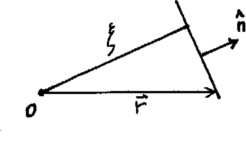
\includegraphics[width=0.4\textwidth]{images/fig_ft1_conduc1.pdf}	 
	\end{center}
	\caption{}
\end{figure} 

\begin{figure}[htb]
	\begin{center}
	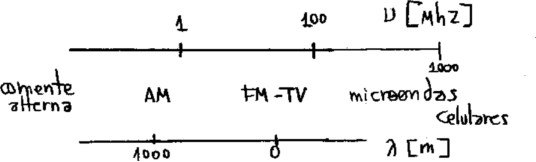
\includegraphics[width=0.4\textwidth]{images/fig_ft1_conduc2.pdf}	 
	\end{center}
	\caption{}
\end{figure} 

\begin{figure}[htb]
	\begin{center}
	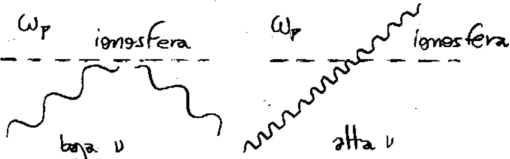
\includegraphics[width=0.4\textwidth]{images/fig_ft1_conduc3.pdf}	 
	\end{center}
	\caption{}
\end{figure} 

\begin{figure}[htb]
	\begin{center}
	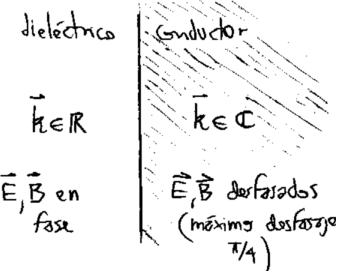
\includegraphics[width=0.4\textwidth]{images/fig_ft1_conduc4.pdf}	 
	\end{center}
	\caption{}
\end{figure} 






% \bibliographystyle{CBFT-apa-good}	% (uses file "apa-good.bst")
% \bibliography{CBFT.Referencias} % La base de datos bibliográfica

\end{document}
